% Unofficial University of Cambridge Poster Template
% https://github.com/andiac/gemini-cam
% a fork of https://github.com/anishathalye/gemini
% also refer to https://github.com/k4rtik/uchicago-poster

\documentclass[final]{beamer}

% ====================
% Packages
% ====================

\usepackage[T1]{fontenc}
\usepackage{lmodern}
\usepackage[size=custom,width=120,height=72,scale=1.05]{beamerposter}
\usetheme{gemini}
\usecolortheme{cam}
\usepackage{graphicx}
\usepackage{booktabs}
\usepackage[numbers]{natbib}
\usepackage{tikz}
\usepackage{pgfplots}
\pgfplotsset{compat=1.14}
\usepackage{anyfontsize}

% ====================
% Lengths
% ====================

% If you have N columns, choose \sepwidth and \colwidth such that
% (N+1)*\sepwidth + N*\colwidth = \paperwidth
\newlength{\sepwidth}
\newlength{\colwidth}
\setlength{\sepwidth}{0.025\paperwidth}
\setlength{\colwidth}{0.3\paperwidth}

\newcommand{\separatorcolumn}{\begin{column}{\sepwidth}\end{column}}

% ====================
% Title
% ====================

\title{Extending Deep Learning Models of Wildfire Spread to Air Quality}

\author{Lorn Jaeger   \and Rupert Williams  \and Kyle Krstulich \and Jake Bova \and Jesse Johnson}

% ====================
% Logo (optional)
% ====================

% use this to include logos on the left and/or right side of the header:
\logoright{
\includegraphics[height=4cm]{AcademicMark.png}}
\logoleft{
\includegraphics[height=10cm]{OUT.png}}

% ====================
% Body
% ====================

\begin{document}

% Refer to https://github.com/k4rtik/uchicago-poster
% logo: https://www.cam.ac.uk/brand-resources/about-the-logo/logo-downloads


\begin{frame}[t]
\begin{columns}[t]
\separatorcolumn

\begin{column}{\colwidth}

  \begin{block}{Introduction}
    The AI/ML research thrust of the SMART Fires project aims to model prescribed fires and their emissions. This poster builds on earlier work predicting next-day wildfire spread, extending the approach to a new target variable, namely PM 2.5, a major component of harmful emissions. The ultimate goal is to be able to do predictions of how prescribed burn emissions will disperse, given information about the area and expected fire spread, helping land managers plan burns that minimize risks to air quality and public health.

  \end{block}


  \begin{block}{Dataset}

The base of the dataset we're training on comes from the WildfireSpreadTS (WSTS) next-day wildfire spread benchmark. WSTS is a collection of 607 U.S. fire events (2018–2021), with data for each day the fire burned, with fields including fuel/vegetation, topography, current and forecasted weather, and landcover. 

\begin{table}[h!]
\centering
\small
\begin{tabular}{l l l p{12cm}}
\toprule
\textbf{Category} & \textbf{Source} & \textbf{Resolution} & \textbf{Feature} \\
\midrule
Vegetation & VIIRS   & 375--750 m & VIIRS bands M11, I2, I1; NDVI; EVI2 \\
\midrule
Weather & GridMET  & 4 km       & Total precipitation; Wind speed and direction; Min/Max temperature; Energy release component; Specific humidity; PDSI \\
\midrule
Topography & USGS & 30 m       & Slope; Aspect; Elevation; Landcover type \\
\midrule
Forecast Weather & GFS & 28 km  & Total precipitation; Wind speed and direction; Temperature; Specific humidity \\
\midrule
Target & VIIRS & 375 m        & Active fire \\
\bottomrule
\end{tabular}
\caption{WildfireSpreadTS Fields}
\end{table}




WSTS improved upon prior datasets by adding multi-day time series inputs and higher temporal resolution paired with high spatial resolution. Our lab has further extended it with several additional years of fires, bringing the total to 1,067 events from 2016-2024.
 

\end{block}

\begin{block}{Selecting a Source of PM 2.5 Data}

  Selecting the best source of PM 2.5 data is not a trivial task. There are many datasets available but they vary in the methods used to produce estimates, usually relying on a combination of physics based models, reanalysis, and satellite measurements of aerosol optical depth. Of these we evaluated four. 
  
  CAMS (Copernicus Atmosphere Monitoring Service) is a global, 3-hourly PM 2.5 forecast from the European Centre for Medium-Range Weather Forecasts that uses the IFS chemistry model, assimilates satellite aerosol optical depth, and reports PM 2.5 directly without sensor correction. MERRA-2 (NASA) is a global GOCART reanalysis where PM 2.5 is calculated from aerosol components; it does not use ground sensors directly. MERRA2R is the same dataset but bias-corrected against AirNow monitors to improve surface accuracy. NCAR (National Center for Atmospheric Research) provides a 12 km CONUS reanalysis using the WRF-CMAQ model that assimilates satellite AOD, designed for higher resolution U.S. air quality. 


\end{block}


  

\end{column}

\separatorcolumn

\begin{column}{\colwidth}

We tested each source by checking it's accuracy relative to a PM 2.5 sensor reading dataset provided by AirNow. 

\begin{figure}
        \centering
        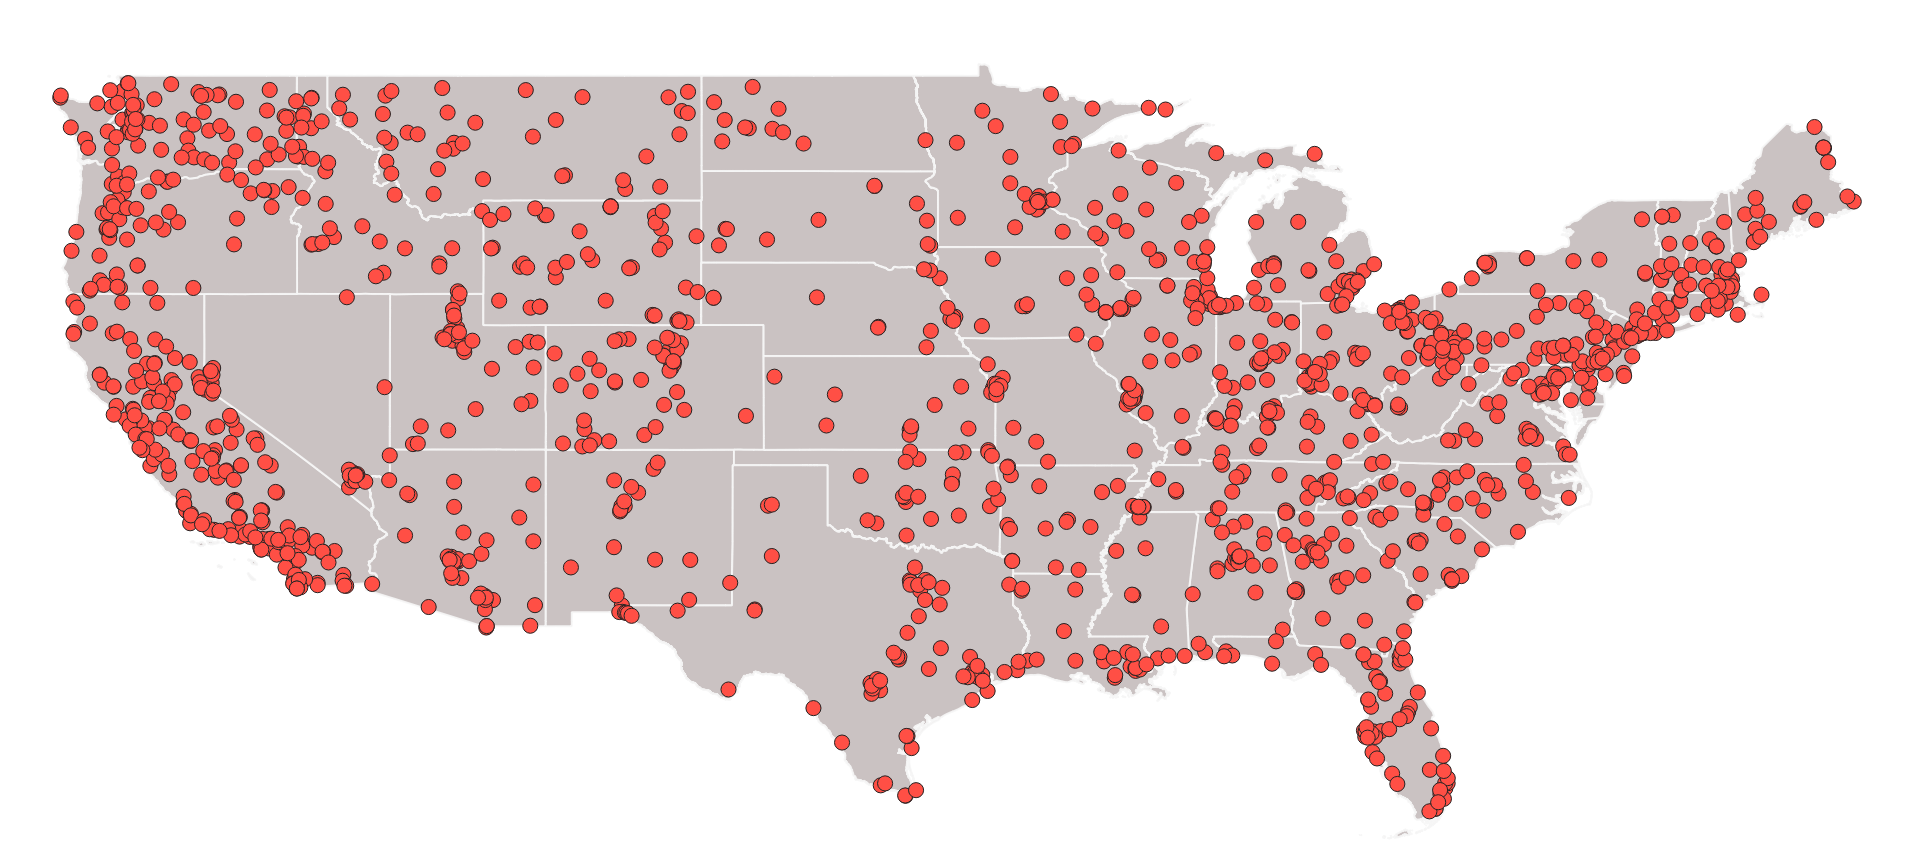
\includegraphics[width=0.5\linewidth]{final_map.png}
        \caption{AirNow sensor locations.}
        \label{fig:placeholder}
\end{figure}




The metrics we really care about are RMSE, which reflects overall accuracy, and slope, which shows how well the dataset scales as PM 2.5 concentrations increase. Because these datasets tend to under predict high PM 2.5 events, a slope closer to 1 means the dataset might better capture the high PM 2.5 coming from a fire.


\begin{table}[h!]
\centering
\small % or \small
\begin{tabular}{lccc}
\toprule
\textbf{Source} & \textbf{Spearman} & \textbf{RMSE} & \textbf{Slope} \\
\midrule
NCAR   & 0.475 & 20.600 & 1.336 \\
CAMS    & 0.352 & 40.890 & 0.189 \\
MERRA2  & 0.426 & 54.019 & 0.166 \\
MERRA2R & \textbf{0.493} & \textbf{20.323} & \textbf{1.071} \\
\bottomrule
\end{tabular}
\caption{Performance metrics by source. Bold values indicate best performance per column.}
\label{tab:placeholder}
\end{table}

MERRA2R outperforms the others in all three metrics while being available globally from 2001-2024, and is what we will be using as a target variable for our training runs.

  \begin{block}{Model Selection \& Training}

  Training a model to predict fire spread is a binary semantic segmentation task, where the input is a multichannel raster made up of the WildfireSpreadTS dataset, the target is a binary mask of the next day's burned pixels, and the output is a raster of probabilities that each pixel burned the next day. To train a model to predict PM 2.5 we will do something similar. Each input will be the same raster but with MERRA2R PM 2.5 added, and a mask of healthy / unhealthy PM 2.5 concentrations (over / under 80 ppm) as the target variable. 

  There are a few options for model architecture. Every architecture is a deep neural net that takes tensor representation of our raster as input, and does some sort of convolution on it, sometimes also using techniques like attention to take advantage of WSTS's temporal component. Previous work has used U-Net, ConvLSTM, SwinUnet, and U-TAE architectures. We ended up using the U-TAE, which had performed the best on the original WildfireSpreadTS dataset.

  \begin{figure}
        \centering
        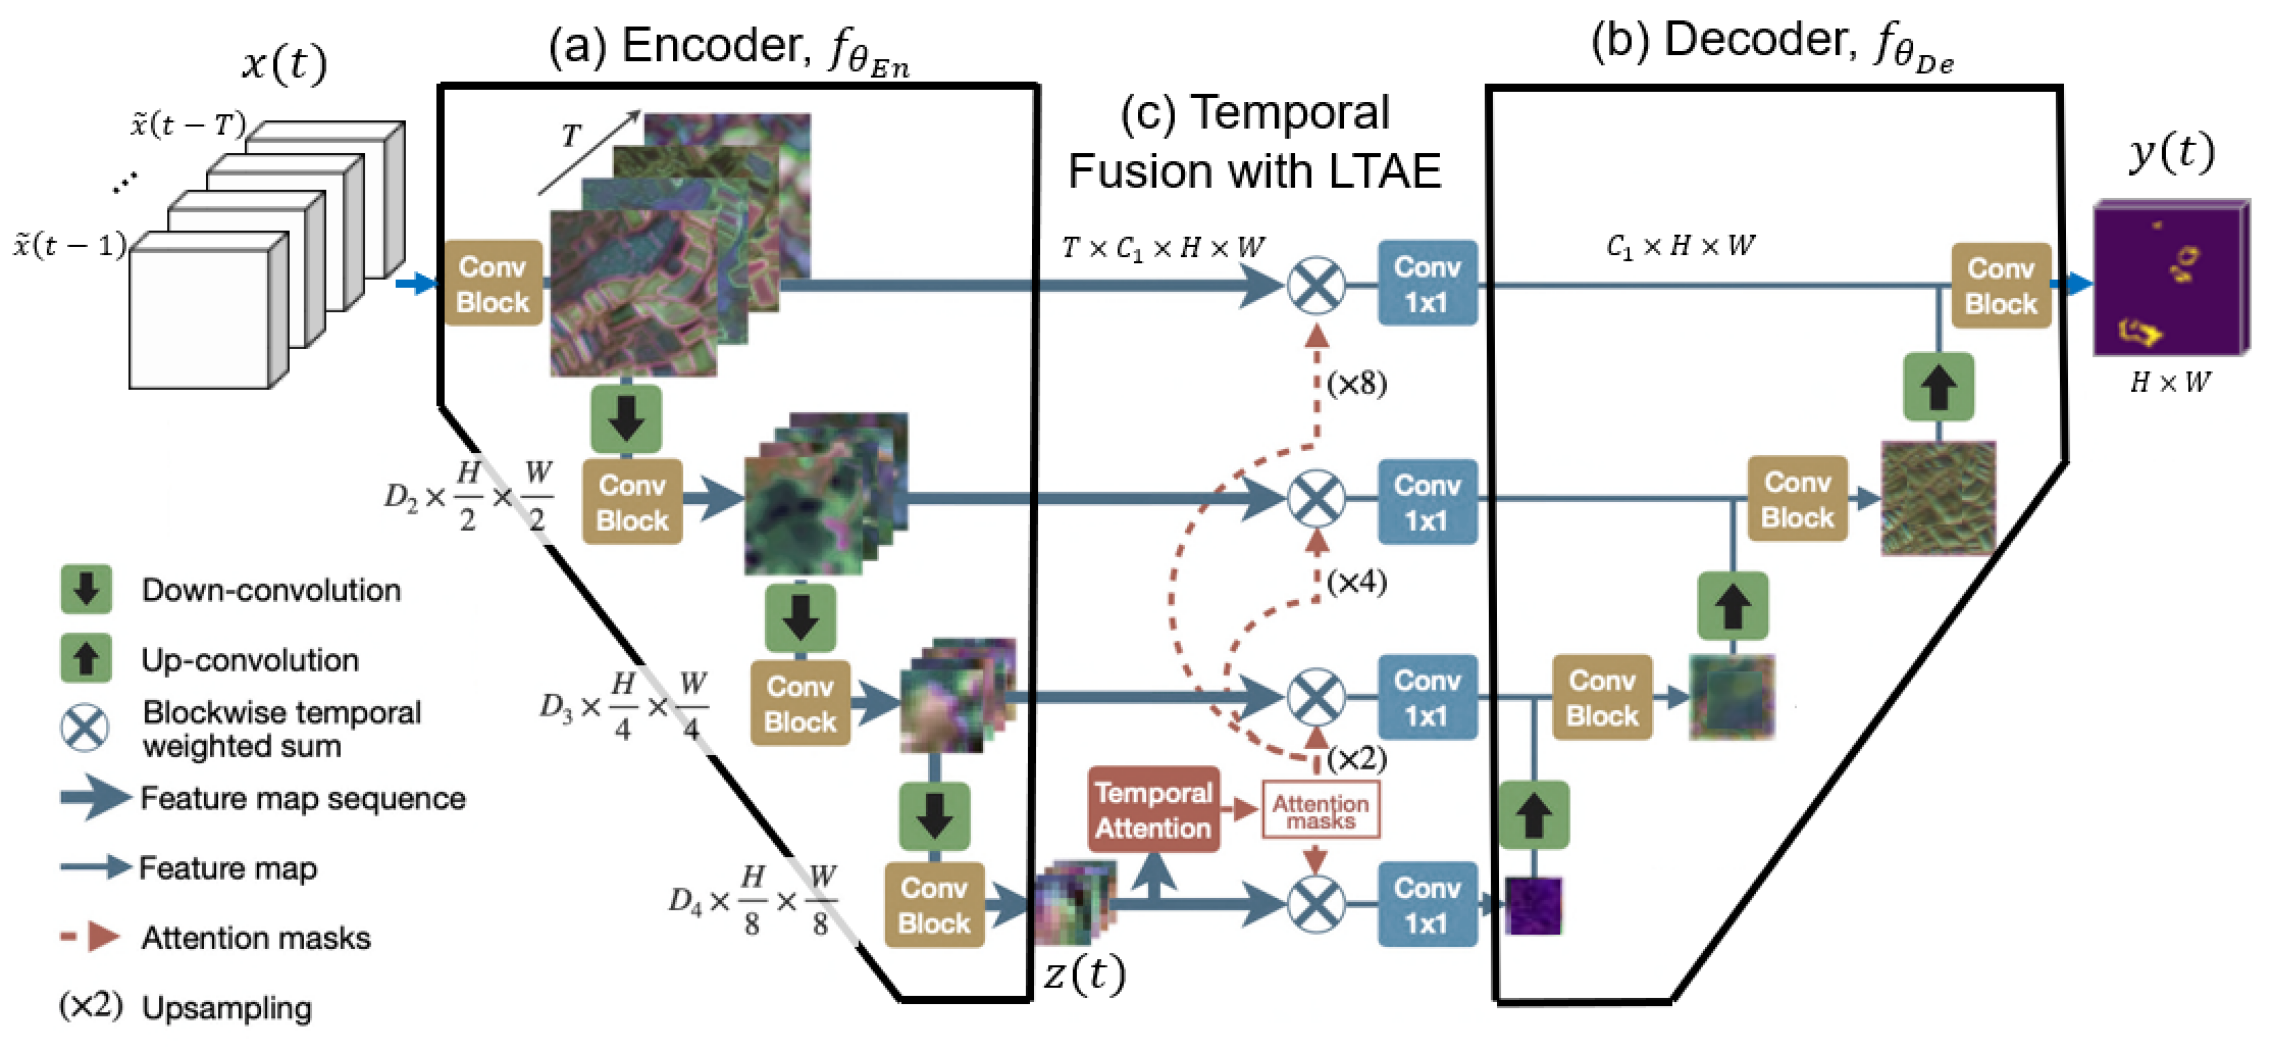
\includegraphics[width=0.6\linewidth]{x2.png}
        \caption{Illustration of the U-Net and UTAE models. If I have permission to use this I will, otherwise there a public domain illustrations of Unets.}
        \label{fig:placeholder}
\end{figure}
 

 

 


\end{block}


\end{column}

\separatorcolumn

\begin{column}{\colwidth}

For training we make use of the setup found by previous modeling improvements by our lab. The previous five days of data are used as input, with dates encoded positionally. Our encoder is initialized with weights from pre-trained Res18 model and our decoder is trained from scratch. We use the previous best learning rate and loss function as well (BCE). Our training split uses data from the year 2020 as a validation set, 2021 as the test set, and the rest of the dataset for training. 




  \begin{block}{Results}

  \begin{itemize}
    \item Naive approach of MERRA2R as a target variable does not really work, the window is too small.
    \item Improvement to naive approach, changing resolutions, different fire encoding, giving next day fire to the model as well, different fields.
\end{itemize}
    

  \end{block}


  \begin{block}{Further Work}
     \begin{itemize}
    \item Discuss results and flaws with approach
    \item Higher quality wind from WRF
    \item More training data in general
    \item Using that flow matching with temporal coherence thing doug was talking about to interpolate between wrf chem and wildfirets
    \item higher quality pm 2.5 data from wrf chem or other

\end{itemize}

  \end{block}

  


 

  

  

\end{column}

\separatorcolumn


\end{columns}
\end{frame}

\end{document}
